\newpage

\section{Формат данных}

\subsection{Проблемы при регистрации ЭЭГ}

После того, как ЭЭГ снято, необходимо отфильтровать сигнал для получения более точных
показателей. Сигнал плохо виден на фоне шума, который создают различные артефакты.
В связи с этим возникает проблема обработки записи --- удаление артефактов для получения
более точных показателей.  

При регистрации ЭЭГ артефактом является любая активность, не связанная с электрической
активностью мозга. Все артефакты и помехи при регистрации ЭЭГ могут быть разделены на две большие группы:
\begin{enumerate}
    \item аппаратные артефакты и внешние помехи физической природы; 
    \item физиологические артефакты, регистрируемые от больного. 
\end{enumerate}
Наиболее частыми являются электродные артефакты и физиологические артефакты,
связанные с регистрацией потенциалов, возникающих при моргании и движении глаз,
миографических потенциалов при мышечном напряжении.  

\subsection{Предварительная обработка данных}

Для удаления артефактов был использованный автоматический метод, реализованный для
среды обработки ЭЭГ (MNE) \cite{MNE}. После предварительной очистки данные ЭЭГ были
отфильтрованы в диапазоне частот 1-30 Гц. Далее с помощью метода Уэлча для стандартных
узких частотных диапазонов ЭЭГ
\begin{itemize}
    \item $\delta:\:$ 1-4 Гц
    \item $\theta:\:$ 4-8 Гц
    \item $\alpha_1:\:$ 8-10 Гц
    \item $\alpha_2:\:$ 10-13 Гц
    \item $\beta_1:\:$ 13-20 Гц
    \item $\beta_2:\:$ 20-30 Гц
\end{itemize}
спектральная мощность сигнала была проанализирована отдельно для тестов Стернберга
разной сложности (3, 4, 5 или 6 цифр и более для запоминания).

После удаления артефактов данные были получены в виде набора .csv файлов. Каждый файл содержал
в себе данные, относящиеся к конкретному человеку и типу задачи (см. главу
\ref{sec:chapter_2_2}),то есть всего 404 файла. Данные из файлов были объединены
в один набор данных, пригодных для обработки алгоритмами машинного обучения.

\subsection{Вид полученных данных}

Полученный набор данных устроен следующим образом (см. рис. \ref{fig_3})\\
\begin{figure}[H]
    \centering
    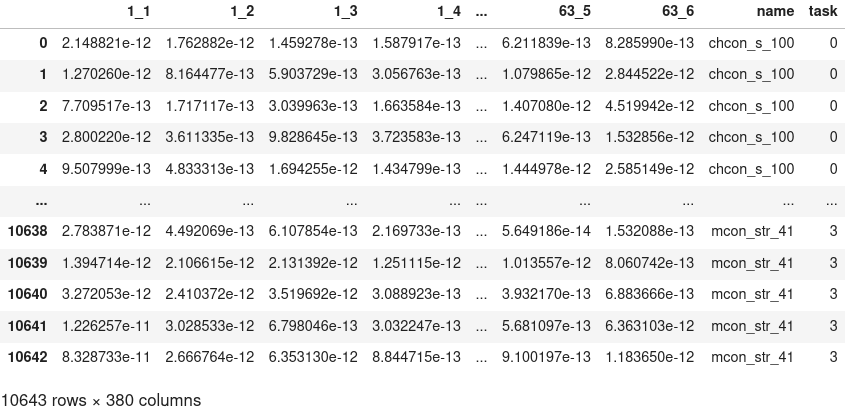
\includegraphics[width=\linewidth]{images/3.png}
    \caption{Полученный набор данных ЭЭГ}
    \label{fig_3}
\end{figure}

Каждый объект выборки --- вектор размерности $63*6+1+1=380$, в котором первые $63*6=378$
столбцов есть амплитуды колебаний электромагнитной активности, которые регистрировались
каждым из 63 электродов (каждый электрод в свою очередь характеризуется шестью частотными
диапазонами спектра). Также есть столбец $"name"$, содержащий идентификатор участника
эксперимента, и столбец $"task"$ с соответствующим типом задачи, которую решал участник во
время снятия ЭЭГ данных. Каждому из 4 типов задачи (лёгкая, средняя, повышенной сложности
и трудная) соответствует число от 0 до 3.

Всего 101 участником эксперимента было решено от 22 до 32 задач каждого из 4 типов сложности.
Суммарное количество объектов в выборке составляет 10641.

Рассмотрим объект выборки более подробно (см. рис. \ref{fig_4}):
\begin{itemize}
    \item \textcolor{red}{Красным цветом} выделены амплитуды колебаний электромагнитной
    активности электродов (каждый из 63 характеризуется шестью частотными диапазонами).
    В каждой ячейке значением является число;
    \item \textcolor{green}{Зелёным цветом} --- идентификатор участника; 
    \item \textcolor{blue}{Синим цветом} --- тип задачи (число от 0 до 3).
\end{itemize}


\begin{figure}[H]
    \centering
    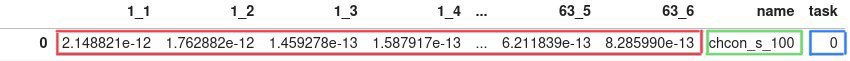
\includegraphics[width=\linewidth]{images/4.png}
    \caption{Детальный вид объекта выборки}
    \label{fig_4}
\end{figure}
